\section{Technical validation}

Validation tests structural, economic and computational properties within specified populations. Readable files, unique identifiers, balanced settlements and reproducible calculations establish different properties; none alone proves complete acquisition or external truth. We distinguish documented checks, direct table checks, historical protocol validation and replay from retained inputs.

\subsection{Structural consistency and economic semantics}

Structural checks examine source identities, native keys, table relationships and lifecycle order. Request-level records and voter-level accounting entries are tested separately because their units differ. Cross-chain checks test whether linked records identify the same protocol object.

Economic classification is checked against the historical implementation, the recorded execution and the financial quantity being measured. For each correction, an object-level record preserves the previous value, the revised value, the source locator and the applied rule. Source binding is strongest for the retained VotingV2 implementation; the OOv2 and Tellor bindings remain qualified, as described in Appendix~\ref{app:semantics}.

Table~\ref{tab:semantic_repair} reports classification errors and corrections for UMA challenges and settlements, Tellor outcomes and DVM penalty accruals. Corrected UMA winner-reward components total 201,500 USDC.e and 1,250 USDC, kept separate by asset. These reclassify existing settlements rather than add payments. Of thirteen Tellor disputes, three support the challenge and have positive applied slashes; ten reject it and have no positive applied slash under the recorded checks. SUPPORT denotes a decision for the disputer.

\begin{table}[!htbp]
\centering\tabstyle
\caption{Economic-semantic checks and correction evidence. Native populations may overlap across rules.}
\label{tab:semantic_repair}
\begin{tabularx}{\linewidth}{@{}L{.19\linewidth}Yrr@{}}
\toprule
Rule & Evidence and interpretation & Population & Before / after \\
\midrule
UMA challenge & Dispute event and nonzero disputer; a proposal alone is insufficient. & 42,676 & 40,992 / 0 \\
UMA settlement & Settled lifecycle and matched token movement. Open requests remain unsettled. & 42,676 & 850 / 0 \\
UMA winner gain & Contract payout rule and settlement transfer; returned principal is separate. & 42,676 & 834 / 0 \\
Tellor outcome & SUPPORT accepts the challenge and rejects the report. & 13 & 13 / 0 \\
Tellor applied loss & Final dispute outcome; initiation escrow is distinct from applied loss. & 13 & 10 / 0 \\
DVM accrual & Signed request accrual; an applied stake change requires separate evidence. & 2,663,684 & 947,128 / 0 \\
\bottomrule
\end{tabularx}
\end{table}


\begin{figure}[!htbp]
\centering
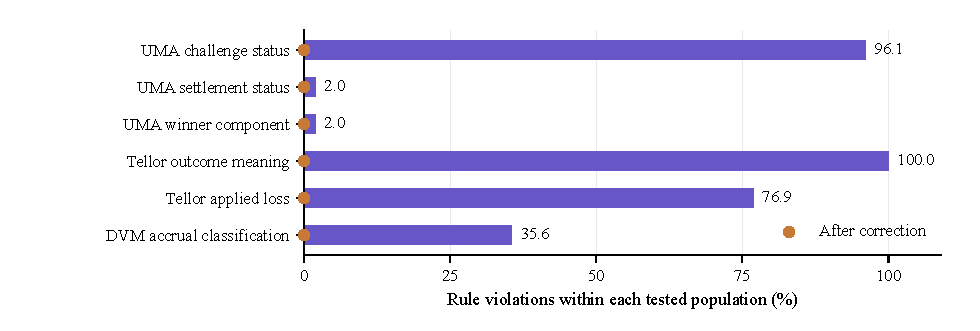
\includegraphics[width=0.99\linewidth]{figures/semantic_gallery.pdf}
\caption{Economic-semantic corrections within six separately defined populations. Bars show the proportion violating each rule before correction; orange markers show the corresponding proportion after applying the rule. Populations and rule evidence are specified in Table~\ref{tab:semantic_repair}. A request may be affected by more than one rule.}
\label{fig:semantic}
\end{figure}


In the DVM population, 947,128 negative accruals had been classified as applied principal losses without evidence of a corresponding reduction. Reclassifying them as penalty accruals preserves the accounting state without asserting realized loss. Valid records still require interpretation under the mechanism's rules.

\subsection{Accounting reconciliation and object identity}

All 41,826 settled UMA requests satisfy the recorded integer payout identity,
\begin{equation}
 \Delta_{\mathrm{payout}}=G_{\mathrm{actual}}-G_{\mathrm{expected}}=0,
 \label{eq:payoutcheck}
\end{equation}
with the associated transfer-matching checks passing under the applicable contract and adapter rules. Chainlink checks identify 51,372 qualified staking and reward records: 50,772 require transfers and match the recorded token movements, while 600 are accounting-only adjustments. The historical Flare report documents Merkle-root and claim reconciliation for 183 closed reward epochs. Those retained results are distinguished from a fresh rerun of the complete chain-level validation.

Of 835 UMA cross-chain link attempts, 832 meet the deterministic Grade-A rule and three remain unmatched. Pyth replay checks reward-state calculations over 49 retained closed epochs. These results support tested links and accounting; completeness, row ancestry and external truth remain unverified.

\subsection{Computational reproducibility}

A worked UMA case links archived events to a request lifecycle and reconciles economic records with token movements. Repeated executions check consistency for identical inputs and code.

These evaluations concern reconstruction from retained evidence. Reacquiring historical data also depends on archive access, interface behaviour and the original collection boundaries. The acquisition records document those conditions separately from the computational checks.

\subsection{Temporal consistency}

Temporal checks compare UTC conversions with native values and verify observation order. Millisecond clocks preserve fractional seconds. Native and UTC selections agree for the tested daily and weekly windows. Epoch checks verify retained boundaries and the assignment of observations at interval endpoints.

Missing timestamps are assessed separately from event absence. Exact block matching improves temporal availability for some EVM records, while unresolved observations retain a missing-time status. Appendix~\ref{app:temporal} summarizes these limitations and the distinction between timestamp availability and historical coverage.


\subsection{Daily aggregation and prediction-task checks}

Daily validation checks that grouped event counts and integer monetary totals agree with their eligible native inputs. Escrow exposure is checked by comparing daily balance-duration totals with the integral over the request's observed transfer intervals. A valid timestamp is required for assignment to a day; eligible observations without one remain in the source population and in the missing-time accounting.

The prediction-task checks examine request uniqueness, cohort membership, target construction and feature timing. Role-history counts and rates are compared with a separate direct selection of prior settlements. The checks also preserve the distinction between a native event observed by the proposal and a historical parameter whose availability requires additional source binding. Feature distributions and missingness are provided in Appendix~\ref{app:prediction} to support inspection of the task data.

\subsection{Worked cross-chain settlement}
\label{sec:case}

The worked dispute links four Polygon transactions to an Ethereum VotingV2 resolution. Polygon records the request, proposal, challenge and local settlement. Checks verify receipt status, blocks, event positions and request identity. Figure~\ref{fig:case} presents timing and cashflows; Appendix~\ref{app:case} lists events and relay gaps.

Proposal occurs about 7.7 hours after the request, followed shortly by a challenge. DVM resolution follows about 92.2 hours later, and Polygon settlement follows after roughly 22 minutes. These endpoints cannot separate transport, scheduling and adjudication. Early expiration retains its nonbinary meaning.

Each party posts 750 USDC.e. The winner receives 1,000 USDC.e: 750 in returned principal and 250 in gain. The fee recipient receives 500. The configured reward is refunded or rolled over separately. Flows balance, but net profit requires costs. Cross-chain identity does not establish a bridge transfer.
\begin{figure}[!htbp]
\centering
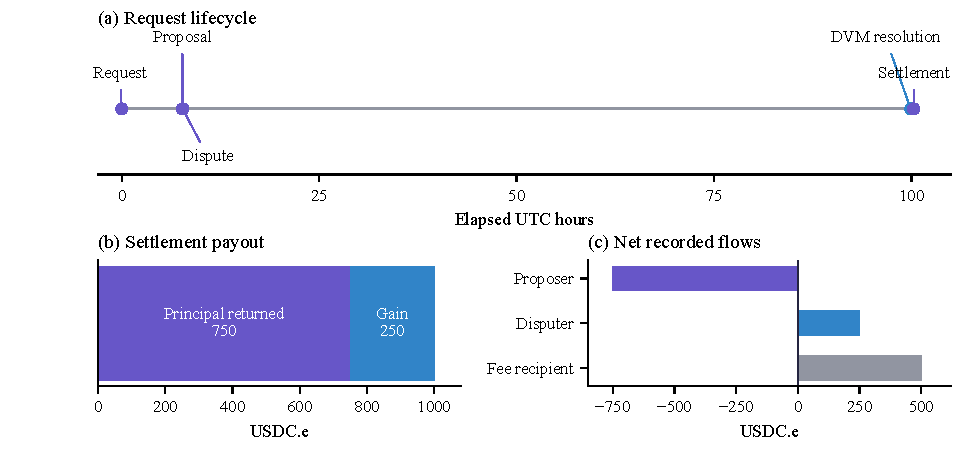
\includegraphics[width=0.99\linewidth]{figures/cross_chain_gallery.pdf}
\caption{A linked UMA dispute. (a) Events on a proportional elapsed-time axis: Polygon events are purple and the Ethereum resolution is blue. The proposal and challenge are close in time. The interval between challenge and resolution includes unobserved intermediate transport steps. (b) The winner's gross payout separates principal from gain. (c) Participant and fee-recipient net flows balance in USDC.e, before additional costs.}
\label{fig:case}
\end{figure}
